% Offizielle Beispieldatei für beamer-Vorlage aus tubslatex Version 0.3alpha2
\documentclass[fleqn,11pt]{beamer}

\usepackage[ngerman]{babel}
\usepackage[utf8x]{inputenc}
\usepackage{graphicx}
\usetheme[%
  %cmyk,%<rgbprint>,          Auswahl des Farbmodells
  blue,%<orange/green/violet> Auswahl des Sekundärfarbklangs
  dark,%<light,medium>        Auswahl der Helligkeit
  %colorhead,%    Farbig hinterlegte Kopfleiste
  %colorfoot,%    Farbig hinterlegt Fußleiste auf Titelseite
  colorblocks,%   Blöcke Farbig hinterlegen
  %nopagenum,%    Keine Seitennumer in Fußzeile
  %nodate,%       Kein Datum in Fußleiste
  tocinheader,%   Inhaltsverzeichnis in Kopfleiste
  %tinytocinheader,% kleines Kopfleisten-Inhaltsverzeichnis
  %widetoc,%      breites Kopfleisten-Inhaltsverzeichnis
  %narrowtoc,%    schmales Kopfleisten-Inhaltsverzeichnis
  %nosubsectionsinheader,%  Keine subsections im Kopfleisten-Inhaltsverzeichnis
  %nologoinfoot,% Kein Logo im Fußbereich darstellen
  ]{tubs}

% Titelseite
\title{AIO - Akustische Indoor-Ortung}
\subtitle{Praktikum Wireless Sensor Networks - Team 4}
\author{Johannes Starosta, Lena Schimmel}
% Titelgrafik, automatisch beschnitten, Weitere Optionen: <scaled/cropx/cropy>
% \titlegraphic[cropped]{\includegraphics{infozentrum.jpg}}
\titlegraphic[scaled]{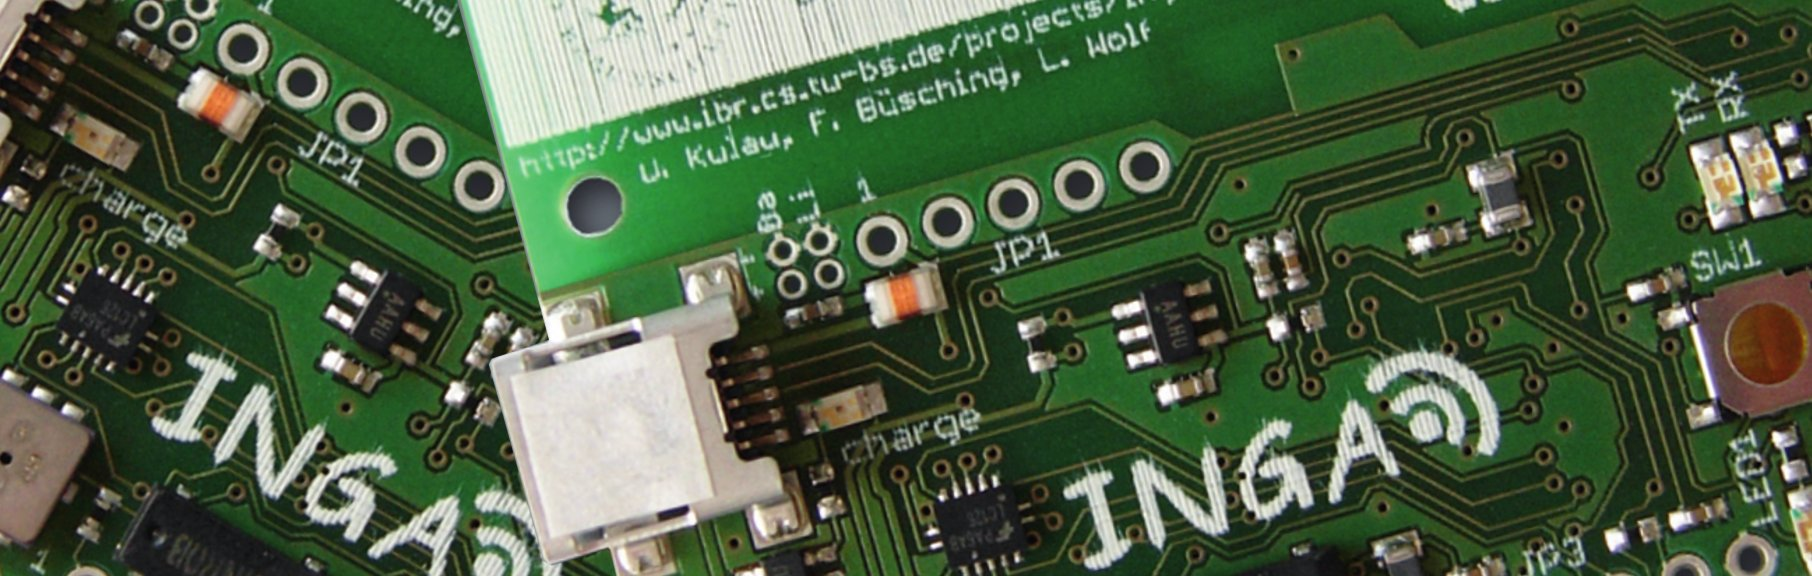
\includegraphics{titlepicture3.jpg}}

% Logo, dass auf Titelseiten oben rechts und auf Inthaltsseiten unten rechts
% dargestellt wird. Es wird jeweils automatisch skliert
\logo{
\includegraphics{ibr.jpg}}
%\logo{Institut für Unkreativität\\und Schreibschwäche}

\begin{document}

\begin{frame}[plain]
\titlepage
\end{frame}


\begin{frame}{Motivation und Ausgangssituation}
Location Based Services sind im Trend. Übliche Technologien:
\begin{itemize}
  \item GPS
  	\begin{itemize}
	  \item Nur unter freiem Himmel
	  \item Genauigkeit ca. 6m
	  \item In den meisten Smartphones, sonst selten
	\end{itemize}
  \item Funkzellenortung / WiFi
  	\begin{itemize}
	  \item Auch in Innenräumen
	  \item Genauigkeit ca. 200m
	\end{itemize}
\end{itemize}
Dabei wäre gerade in Innenräumen eine mindestens Meter-genaue Ortung wünschenswert.
\end{frame}

\begin{frame}{Idee}
	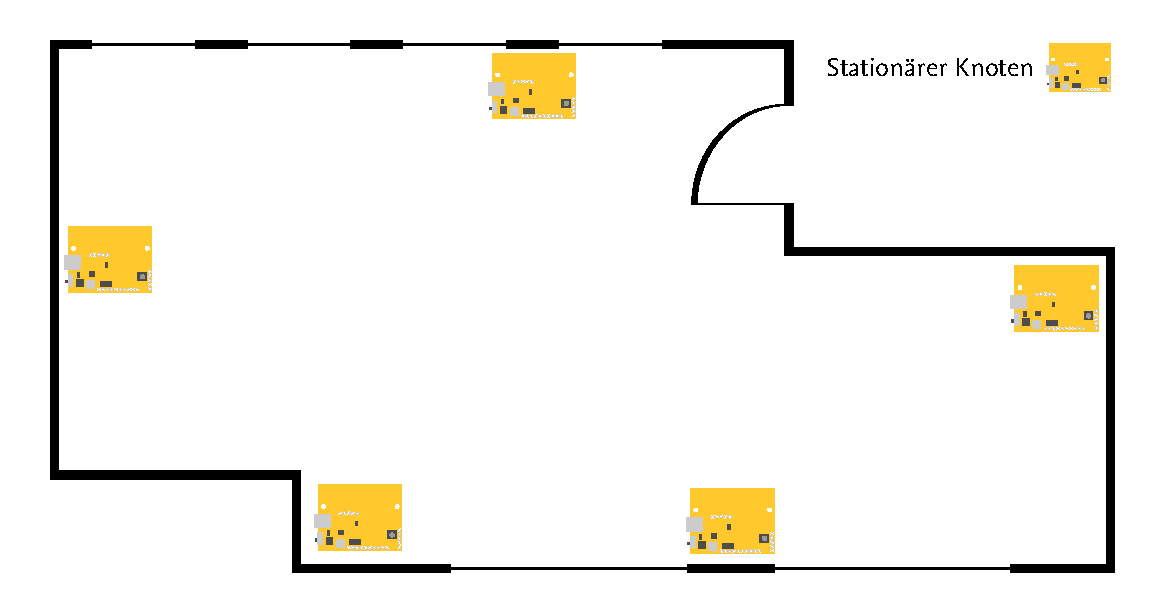
\includegraphics[width=1.0\textwidth]{room-1.pdf}
	
	Knoten werden stationär im Raum verteilt.
\end{frame}


\begin{frame}{Idee}
	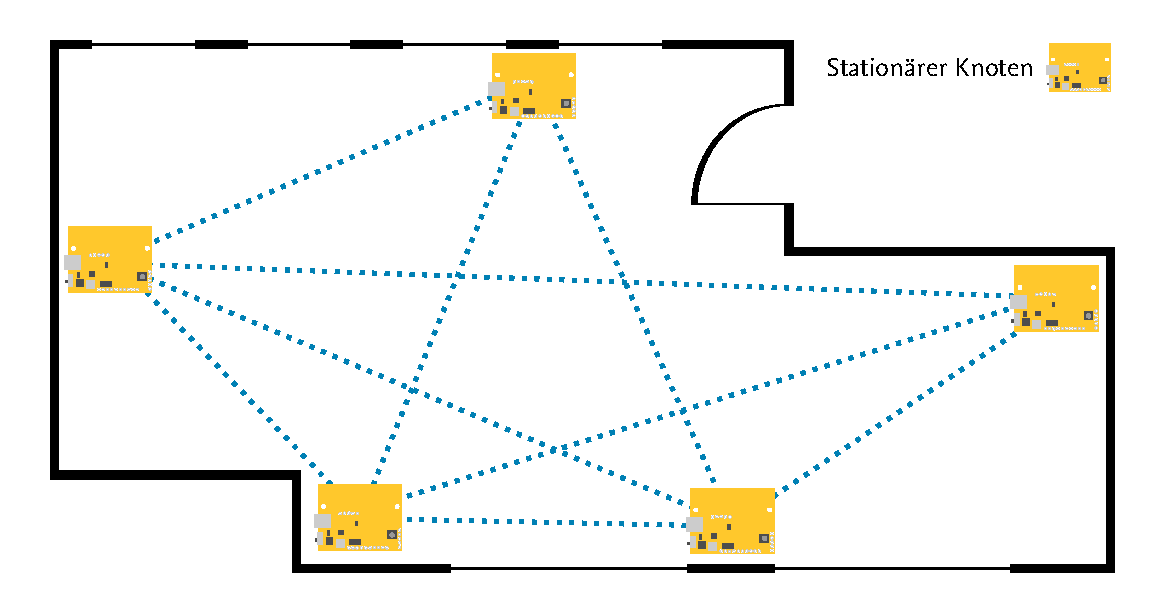
\includegraphics[width=1.0\textwidth]{room-2.pdf}

	Diese vermessen automatisch ihre Abstände und relative Lage.
\end{frame}


\begin{frame}{Idee}
	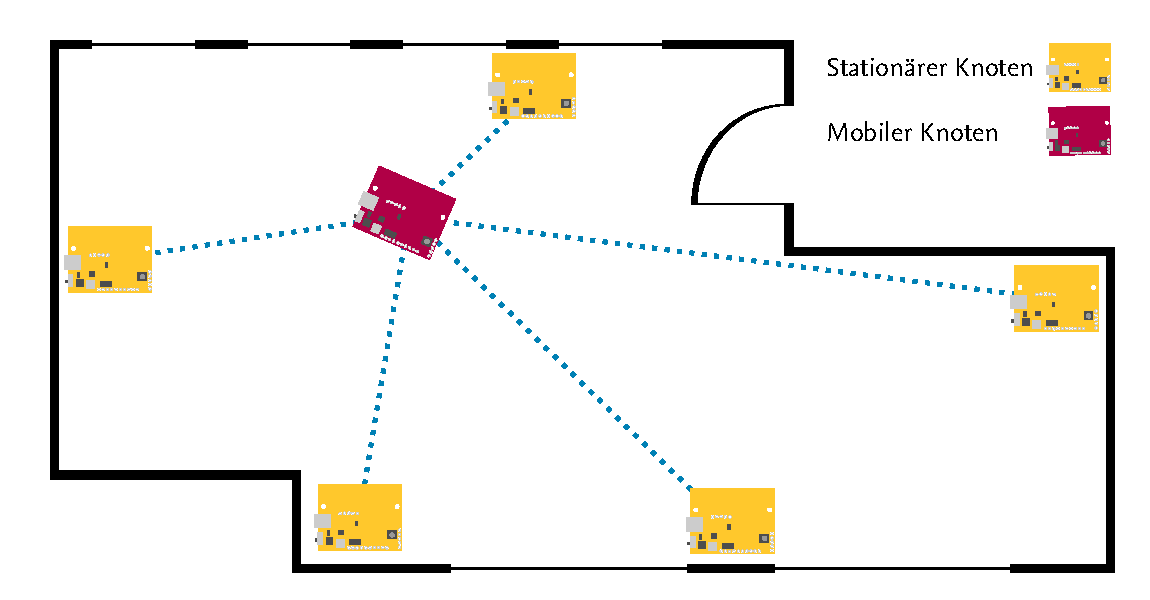
\includegraphics[width=1.0\textwidth]{room-3.pdf}

	Mobile Knoten können ihre Lage im Raum bestimmen.
\end{frame}


\begin{frame}{Idee}
	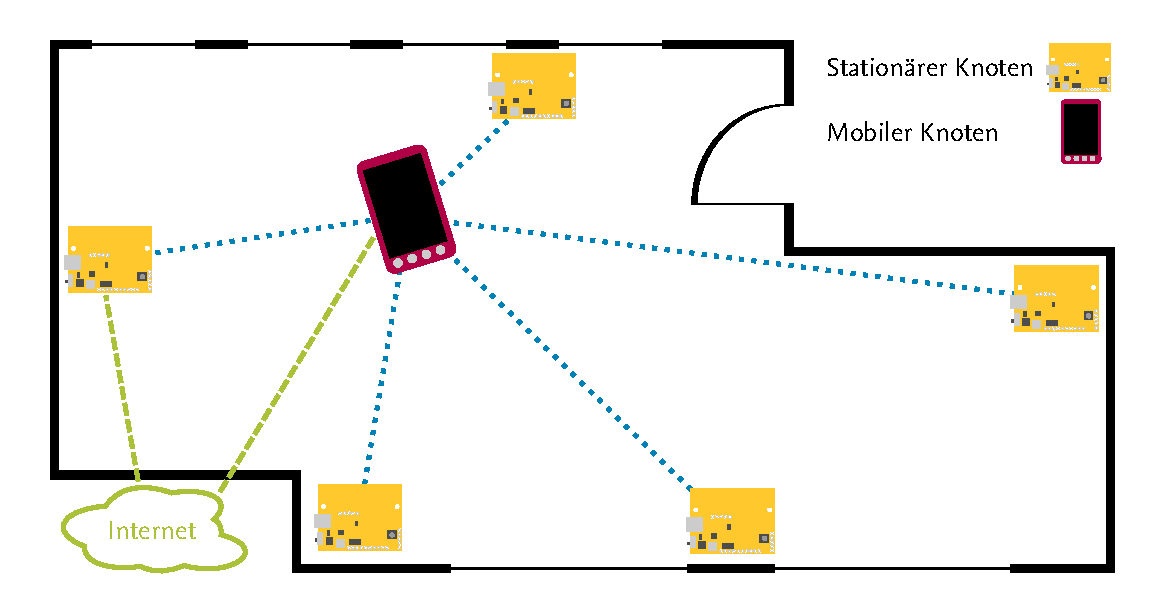
\includegraphics[width=1.0\textwidth]{room-4.pdf}

	Dies kann auch mit Standard-Hardware geschehen.
\end{frame}

\begin{frame}{Idee - zusammengefasst}
\begin{itemize}
  \item Kommunikation und Synchronisation über Funk
  \item Distanzmessung über Schall
  \item Frequenz: 22kHz
  \item Genauigkeit: wenige Zentimeter (theoretisch)
  \item Ortungsintervall: mehrmals pro Sekunde
\end{itemize}
\end{frame}

\begin{frame}{Anforderungen / Arbeitspakete}
\begin{itemize}
  \item Hardware zur Audio-Ein- und -Ausgabe
  \item Zeitsynchronisation über Funk
  \item Koordination der Sendezeitpunkte
  \item Laufzeitbestimmung
  \item Relative Lage aus Abständen errechnen
  \item Visualisierung der Lage(n)
  \item Fallback über Audio-Fingerprints
\end{itemize}
\end{frame}

\end{document}
